\documentclass[10pt]{article}

%==============================
% Document Metadata
%============================== 
\usepackage[pdftex,
    pdfauthor={Rukmal Weerawarana},
    pdftitle={Homework 1 Solutions - FE 621},
    pdfsubject={FE 621 - Computational Methods in Finance}
]{hyperref}


%==============================
% Package Imports
%==============================    
\usepackage[ruled]{algorithm2e} % typeset algorithms
\usepackage[authordate, maxcitenames=1]{biblatex-chicago} % chicago bibliography style
\usepackage{amsmath} % math environment stuff
\usepackage{amssymb} % additional math symbols
\usepackage[toc, page]{appendix} % Appendix referencing
\usepackage{booktabs} % Table lines
\usepackage{comment} % enables the use of multi-line comments (\ifx \fi)
\usepackage[skip=5pt, labelfont=bf]{caption} % caption formatting
\usepackage{csvsimple} % CSV import to Table
\usepackage{fancyhdr} % Header
\usepackage{fancyvrb} % Verbatim text
\usepackage{float} % Controlling figure border
\usepackage[headings]{fullpage} % Set all margins to 1.5 cm
\usepackage{graphicx} % Figures
\usepackage{listings} % code embedding
\usepackage{longtable} % Multipage tables
\usepackage{multirow} % Multirow cells in tables
\usepackage{pmboxdraw} % Box characters for file tree
\usepackage[dvipsnames]{xcolor} % colors for code


%==============================
% Configuration
%==============================

% Figure outline configuration
% \floatstyle{boxed}
% \restylefloat{figure}

% Bibliography configuration

\addbibresource{../bibliography.bib}

% Remapping bibliography underscores (_) and tildes (~) because Mendeley has weird exporting
% Solution from: https://tex.stackexchange.com/questions/309980/parsing-underscores-in-urls-from-mendeley

\DeclareSourcemap{ % Used when .bib/Bibliography is compiled, not when document is
    \maps{
        \map{ % Replaces '{\_}', '{_}' or '\_' with just '_'
            \step[fieldsource=url,
                  match=\regexp{\{\\\_\}|\{\_\}|\\\_},
                  replace=\regexp{\_}]
        }
        \map{ % Replaces '{'$\sim$'}', '$\sim$' or '{~}' with just '~'
            \step[fieldsource=url,
                  match=\regexp{\{\$\\sim\$\}|\{\~\}|\$\\sim\$},
                  replace=\regexp{\~}]
        }
    }
}

% Code display configuration

\newcommand*\lstinputpath[1]{\lstset{inputpath=#1}} % Setting path
\lstset{
	language=Python,
	basicstyle=\footnotesize\ttfamily,
	commentstyle=\ttfamily\color{purple!40!black},
	identifierstyle=\color{blue},
	keywordstyle=\color{ForestGreen},
	numbers=left,
	numberstyle=\ttfamily\color{gray}\footnotesize,
	stepnumber=1,
	numbersep=5pt,
	backgroundcolor=\color{white},
	showspaces=false,
	showstringspaces=false,
	showtabs=false,
	frame=single,
	tabsize=2,
	captionpos=b,
	breaklines=true,
	breakatwhitespace=false,
	title=\lstname
}
\lstset{
	language=R,
	basicstyle=\footnotesize\ttfamily,
	commentstyle=\ttfamily\color{purple!40!black},
	identifierstyle=\color{blue},
	keywordstyle=\color{ForestGreen},
	numbers=left,
	numberstyle=\ttfamily\color{gray}\footnotesize,
	stepnumber=1,
	numbersep=5pt,
	backgroundcolor=\color{white},
	showspaces=false,
	showstringspaces=false,
	showtabs=false,
	frame=single,
	tabsize=2,
	captionpos=b,
	breaklines=true,
	breakatwhitespace=false,
	title=\lstname
}

% Header and Footer configuration

\pagestyle{fancy} % set page style
\fancyhead{} % override header
\fancyfoot{} % override footer
\renewcommand{\headrulewidth}{.4pt} % set header rule width 
\renewcommand{\footrulewidth}{.4pt} % set footer rule width 
\lhead{Homework Assignment 2} % set left header
\rhead{Rukmal Weerawarana} % set right header
\lfoot{\textit{FE 621}: Computational Methods in Finance} % set left footer
\rfoot{Page \thepage} % set right footer


%==============================
% Document Content
%==============================

\begin{document}

\thispagestyle{plain}

\pagenumbering{roman}  % Changing numbering to Roman numerals for first pages

%==============================
% Document Title
%==============================

\noindent
\large\textbf{Homework Assignment 2} \hfill \textbf{Rukmal Weerawarana} \\
\normalsize \textit{FE 621}: Computational Methods in Finance \hfill \textit{rweerawa@stevens.edu} $\mid$ 104-307-27 \\
\textit{Instructor}: Ionut Florescu \hfill Department of Financial Engineering \\
3/25/2019 \hfill Stevens Institute of Technology

\noindent\rule{\linewidth}{.1em}


%==============================
% Overview
%==============================

\section*{Overview}

In this Homework Assignment, we explore various tree construction methods, and price various option contracts. I implement a highly generalized Tree, that is extended and utilized throughout the assignment.

Unless otherwise stated, data is from the same dataset used in Homework 1:

\begin{itemize}
    \item \textbf{DATA2} - Thursday, February 7 2019 (\textit{2/7/19}).
\end{itemize}

The content of this Homework Assignment is divided into four sections; the first discusses tree construction. The second contains various computations with the Trigeorgis Binomial Tree, and the third discusses additive Trinomial pricing trees. Finally, the fourth section explores the pricing of exotic options with trees.

\begin{center}
    \textit{See Appendix~\ref{appendix:source} for specific question implementations, and the project GitHub repository\footnote{\cite{Weerawarana2019}} for full source code of the {\normalfont \texttt{fe621}} Python package.}
\end{center}


%==============================
% Table of Contents
%==============================

\newpage

\tableofcontents

%==============================
% Section 1
%==============================

\newpage

\pagenumbering{arabic}  % Changing numbering to arabic numerals for main content

\section{Tree Implementation}

    \subsection{General Tree Construction} \label{section:gen_tree}

    To simplify the construction of all tree-like structures, I implemented a fully generalized tree structure. This structure handles tree construction and traversal, completely encapuslating all required functionality.

    The class intelligently exposes price and value tree variables during traversal, and abstract methods are designed to be overridden to implement a specific tree pricing algorithm. This general tree class is reproduced below. Furthermore, the class also utilizes DOK (i.e. \textit{Dictionary-of-Keys}) matrices whenever possible. This provides quick \textit{O(1)} access to elements, and minimizes overall space complexity, as zero-valued fields are not store explicitly.

        \lstinputlisting{../fe621/tree_pricing/general_tree.py}
    

    \newpage
    \subsection{Binomial Tree}

    Following this implementation strategy, the additive Trigeorgis\cite{Trigeorgis1991} tree was implemented. Required methods of the abstract \texttt{GeneralTree} class were overridden to implement the Trigeorgis tree for both Call and Put options, of both American and European options in a single class.

    Furthermore, optimizations were made to the Trigeorgis tree class, such that a European option can be computed from the same price tree as constructed for an American option, and vice versa. This functionality enables efficient cross-style option value computations with minimal space complexity.

    The Trigeorgis tree implementation is reproduced below.

        \lstinputlisting{../fe621/tree_pricing/binomial/trigeorgis.py}

    \newpage
    \subsection{Trinomial Tree}

    
    Similar to the Trigeorgis tree above, a generalized additive Trinomial tree was implemented utilizing the same abstract \texttt{GeneralTree} class. The implementation of a Trinomial tree utilizing the same abstract class illustrates its versatility, with constructed DOK price and value trees intelligently adapting to the different degree of the tree.
    
    This was accomplished entirely by overriding prescribed abstract methods of the \texttt{GeneralTree} class, without any direct modification of the generalized tree class. The Trinomial Additive Tree implementation is reproduced below.

    \lstinputlisting{../fe621/tree_pricing/trinomial/trinomial_price.py}
    
\newpage
\section{Binomial Tree Operations}

    \subsection{Computed Option Prices}

    Option prices were computed, utilizing data from Homework Assignment 1's SPY \textbf{DATA2} dataset. To begin, both American and European style options were computed for options of various strike prices, with expiration dates varying from 1 to 3 months of the data gathering date.

    This data is reproduced in Appendix~\ref{appendix:q1:binomial_prices}, and the source code for this computation is reproduced in Appendix~\ref{appendix:q1:binomial_prices}.

    As seen in the tables, the computed values for the European style option with the Binomial tree agree with the analytically computed Black Scholes price. This behavior is to be expected, as the Binomial Tree price converges to the Black Scholes price as the step size, $N \rightarrow \infty$.

    Furthermore, it can also be noted that the prices of the American style options are consistently higher. Note that some significant figures may be truncated in the presentation of the table in this document.
    
    This behavior is also expected. Under the efficient market hypothesis, and the risk-neutral assumption of option pricing, risk is compensated equally. Thus, the higher cost of the American style options can be attributed to the fact that the holder must pay for the \textit{optionality} provided by the early-exercise feature of American style options, compared to their European style counterparts.


    \subsection{Absolute Error Analysis}
    
    To better understand the behavior of the Binomial Tree pricing under varying step sizes, the following error function was plotted for various values of the step size, $N$. The source code for this computation is reproduced in Appendix~\ref{appendix:source:q1:abs_error}.

    \begin{gather*}
        N \in \{10, 20, 30, 40, 50, 100, 150, 200, 250, 300, 350, 400\} \\
        \\
        \epsilon_N = \left| P^{BSM}(\cdot) - P^{BTree}_N(\cdot) \right|
    \end{gather*}

    \begin{table}[!h]
        \centering
        \csvautotabular{bin/binomial_tree_abs_error.csv}
        \caption{Absolute error of Binomial Tree Put Option price computation, with respect to a range of varying step sizes, $N$.}
        \label{table:binomial_abs_error}
    \end{table}

    Where $P^{BTree}_N$ is the price of a put option computed with a binomial tree of $N$ steps. The table of absolute errors is reproduced in Table~\ref{table:binomial_abs_error}. Additionally, a graphical representation of this data is also presented in Figure~\ref{fig:binomial_abs_error}.

    \begin{figure}[!ht]
        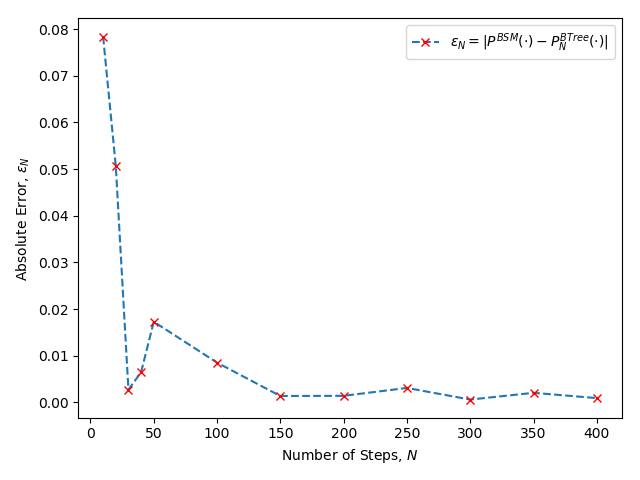
\includegraphics[]{bin/binomial_abs_error_plot.png}
        \caption{Absolute error analysis of the Binomial Tree price computation convergence, with respect to varying step sizes.}
        \label{fig:binomial_abs_error}
    \end{figure}

    As evidenced by the graphic, there is a clear pattern of convergence to a the analytically computed value as the number of steps, $N$ increases. This is to be expected, as at the limit as $N \rightarrow \infty$, the Binomial Tree process will perfectly approximate a continuous geometric brownian motion.

    \newpage
    \subsection{Implied Volatility Computation}
    
    Following the algorithm outlined in Homework 1, I computed the implied volatility for the selection of option contracts used in this Homework Assignment, using the Binomial Option Tree, driven by a Bisection Search Algorithm. Source code for this computation is reproduced in Appendix~\ref{appendix:source:q1:imp_vol}.

    Compared to the implied volatilities computed in Homework Assignment 1, the volatilities computed here are marginally higher. This too can be attributed to the fact that the holder is compensated fairly for the added optionality provided under the American Option heuristic, used in this computation.


    \newpage
    \section{Trinomial Tree Operations}
    
        \subsection{Arbitrary Option Price Computation}

        As outlined in the question, the Trinomial Tree was utilized to compute the price of an option with both Call and Put types, under both the European and American pricing heuristic. The parameters of this option were as follows:

        \begin{gather*}
            S_0 = 100 \\
            K = 100 \\
            T = 1 \\
            \sigma = 25\% \\
            r = 6\% \\
            \delta = 0.03 \\
            \text{With the convergence condition, } \Delta x \geq \sigma \sqrt{3 \Delta t}
        \end{gather*}

        \begin{table}[!h]
            \centering
            \csvautotabular{bin/trinomial_arbitrary_price.csv}
            \caption{Arbitrary option computation with the Trinomial tree.}
            \label{table:trinomial_arb_price}
        \end{table}
    

        The results of this computation are presented in Table~\ref{table:trinomial_arb_price}, and the corresponding source code is reproduced in Appendix~\ref{appendix:source:q2:arb_price}.

        As seen in the previous cases, the price of the American style option is consistently higher than that of its European style counterpart. Again, this is due to the added optionality provided by the American Option pricing heuristic.

        \newpage
        \subsection{Computed Option Prices}
    
        Option prices were computed, utilizing data from Homework Assignment 1's SPY \textbf{DATA2} dataset. To begin, both American and European style options were computed for options of various strike prices, with expiration dates varying from 1 to 3 months of the data gathering date.
    
        This data is reproduced in Appendix~\ref{appendix:q2:trinomial_prices}, and the source code for this computation is reproduced in Appendix~\ref{appendix:q2:trinomial_prices}.
    
        As seen in the tables, the computed values for the European style option with the Trinomial tree agree with the analytically computed Black Scholes price. This behavior is to be expected, as the Trinomial Tree price converges to the Black Scholes price as the step size, $N \rightarrow \infty$.
    
        Furthermore, it can also be noted that the prices of the American style options are consistently higher. Note that some significant figures may be truncated in the presentation of the table in this document.
        
        As with the Binomial Option, this behavior is also expected. Under the efficient market hypothesis, and the risk-neutral assumption of option pricing, risk is compensated equally. Thus, the higher cost of the American style options can be attributed to the fact that the holder must pay for the \textit{optionality} provided by the early-exercise feature of American style options, compared to their European style counterparts.
    
    
        \subsection{Absolute Error Analysis}
        
        To better understand the behavior of the Trinomial Tree pricing under varying step sizes, the following error function was plotted for various values of the step size, $N$. The source code for this computation is reproduced in Appendix~\ref{appendix:source:q2:abs_error}.
    
        \begin{gather*}
            N \in \{10, 20, 30, 40, 50, 100, 150, 200, 250, 300, 350, 400\} \\
            \\
            \epsilon_N = \left| P^{BSM}(\cdot) - P^{TTree}_N(\cdot) \right|
        \end{gather*}
    
        \begin{table}[!h]
            \centering
            \csvautotabular{bin/trinomial_tree_abs_error.csv}
            \caption{Absolute error of Trinomial Tree Put Option price computation, with respect to a range of varying step sizes, $N$.}
            \label{table:trinomial_abs_error}
        \end{table}
    
        Where $P^{TTree}_N$ is the price of a put option computed with a trinomial tree of $N$ steps. The table of absolute errors is reproduced in Table~\ref{table:trinomial_abs_error}. Additionally, a graphical representation of this data is also presented in Figure~\ref{fig:trinomial_abs_error}.
    
        \begin{figure}[!ht]
            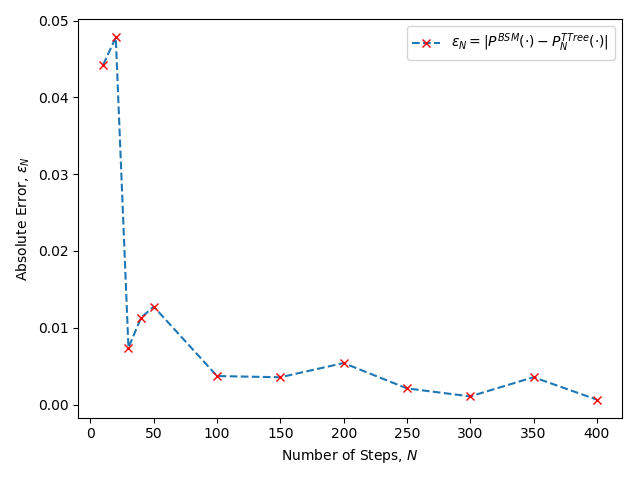
\includegraphics[]{bin/trinomial_abs_error_plot.png}
            \caption{Absolute error analysis of the Trinomial Tree price computation convergence, with respect to varying step sizes.}
            \label{fig:trinomial_abs_error}
        \end{figure}
    
        As evidenced by the graphic, there is a clear pattern of convergence to a the analytically computed value as the number of steps, $N$ increases. This is to be expected, as at the limit as $N \rightarrow \infty$, (similar to the Binomial Tree), the Trinomial Tree process will perfectly approximate a continuous geometric brownian motion.
    
        \newpage
        \subsection{Implied Volatility Computation}
        
        Following the algorithm outlined in Homework 1, I computed the implied volatility for the selection of option contracts used in this Homework Assignment, using the Trinomial Option Tree, driven by a Bisection Search Algorithm. Source code for this computation is reproduced in Appendix~\ref{appendix:source:q1:imp_vol}.
    
        Compared to the implied volatilities computed in Homework Assignment 1, the volatilities computed here are marginally higher. This too can be attributed to the fact that the holder is compensated fairly for the added optionality provided under the American Option heuristic, used in this computation.

        Furthermore, the implied volatilities computed here were also higher compared to their Binomial counterparts. This too is to be expected, as we were evaluating the differing recombination strategies to the same analytical price, thus implying that the given implied volatility was distributed across a larger range of possible price paths.

\newpage
\section{Exotic Option Pricing}

    \subsection{Barrier Option Tree Description}

    In this section, we explore the power of tree pricing methods through the lens of exotic option pricing. Specifically, we attempt to price a series of Barrier options, using a Binomial tree, and standard barrier conditions.

    As with the Binomial and Trinomial tree, this exotic option pricing tree class too was built on the abstract \texttt{GeneralTree} class discussed in Section~\ref{section:gen_tree}.

    The implementation of this class builds on the extreme generality and extensibility of the `GeneralTree` class I designed above. It intelligently modifies the control flow of the standard `GeneralTree' class (functionality provided by design) to price all variants of Put and Call type, Up and Down barrier, In and Out barrier type options, under both American and European pricing heuristics.

    The `Barrier` class utilizes Python's multiple inheritance to its advantage, maintaining - in some cases - two simultaneous trees to utilize \textit{In-Out} Parity to compute In barrier type options. Furthermore, as this builds on the excellent scalability of the DOK matrix-driven `GeneralTree` class, it is extremely space efficient, and provides access to tree nodes in $O(1)$ time complexity.

    \newpage
    \subsection{Barrier Option Tree Source Code}

    The full source code for the Barrier Option Binomial Tree is reproduced below. Note that it inherits `GeneralTree`, discussed in depth in Section~\ref{section:gen_tree}.

    \lstinputlisting{../fe621/tree_pricing/binomial/barrier.py}

    \newpage
    \subsection{Analytical Barrier Option Pricing}

    Additionally, the analytical formula for computing the price of a barrier option were also implemented. This source code is reproduced below.

    \lstinputlisting{../fe621/black_scholes/barrier/call.py}

    \newpage
    \subsection{Barrier Option Computation}

    Here, I present a table with options computed using my Tree implementation, \textit{In-Out} parity, and the analytical formula. The parameters of the computed options are as follows:

    \begin{gather*}
        S_0 = 10 \\
        K = 10 \\
        T = 0.3 \\
        \sigma = 0.2 \\
        r = 0.01 \\
        H = 11 \\
        N = 200
    \end{gather*}

    \begin{table}[!h]
        \centering
        \csvautotabular{bin/barrier_option_values.csv}
        \caption{Values of various barrier options, computed with my Barrier Option Tree, \textit{In-Out} parity, and the analytical formula.}
        \label{table:barrier_options}
    \end{table}

%==============================
% References
%==============================

\newpage

\printbibliography

%==============================
% APPENDIX
%==============================

\newpage

\appendix

% Resetting input path
\lstinputpath{}

\section{Binomial Tree Option Prices} \label{appendix:q1:binomial_prices}

    \csvreader[
        longtable=l|ccccc,
        table head=
            \toprule\bfseries Option Name &\bfseries Strike &\bfseries Implied Volatility &\bfseries Binomial (A) &\bfseries Binomial (E) &\bfseries BS (E) \\ \midrule \endhead \bottomrule \endfoot,
        late after line=\\
    ]{bin/binomial_data2_prices.csv}{1=\one, 2=\two, 3=\three, 4=\four, 5=\five, 6=\six, 7=\seven}{\one & \seven & \five & \two & \three & \four}

\newpage
\section{Binomial Tree Implied Volatility} \label{appendix:q1:imp_vol}

    \csvreader[
        longtable=l|ccc,
        table head=
            \toprule\bfseries Option Name &\bfseries Strike &\bfseries Type &\bfseries Binomial Implied Volatility \\ \midrule \endhead \bottomrule \endfoot,
        late after line=\\
    ]{bin/binomial_implied_vol.csv}{1=\one, 2=\two, 3=\three, 4=\four}{\one & \three & \three & \two}

\newpage
\section{Trinomial Tree Option Prices} \label{appendix:q2:trinomial_prices}

    \csvreader[
        longtable=l|ccccc,
        table head=
            \toprule\bfseries Option Name &\bfseries Strike &\bfseries Implied Volatility &\bfseries Trinomial (A) &\bfseries Trinomial (E) &\bfseries BS (E) \\ \midrule \endhead \bottomrule \endfoot,
        late after line=\\
    ]{bin/trinomial_data2_prices.csv}{1=\one, 2=\two, 3=\three, 4=\four, 5=\five, 6=\six, 7=\seven}{\one & \five & \three & \six & \seven & \two}

\newpage
\section{Trinomial Tree Implied Volatility} \label{appendix:q2:imp_vol}

    \csvreader[
        longtable=l|ccc,
        table head=
            \toprule\bfseries Option Name &\bfseries Strike &\bfseries Type &\bfseries Binomial Implied Volatility \\ \midrule \endhead \bottomrule \endfoot,
        late after line=\\
    ]{bin/trinomial_implied_vol.csv}{1=\one, 2=\two, 3=\three, 4=\four}{\one & \two & \four & \three}

\newpage
\section{Solution Source Code} \label{appendix:source}

    \subsection{Question 1 Implementation} \label{appendix:source:q1}

        \subsubsection{Binomial Tree Price Computation} \label{appendix:source:q1:prices}

            \lstinputlisting{question_solutions/question_1_prices.py}
        
        \subsubsection{Binomial Tree Absolute Error Analysis} \label{appendix:source:q1:abs_error}

            \lstinputlisting{question_solutions/question_1_abs_error.py}
        
        \subsubsection{Binomial Tree Implied Volatility Optimization} \label{appendix:source:q1:imp_vol}

            \lstinputlisting{question_solutions/question_1_imp_vol.py}

    \newpage
    \subsection{Question 2 Implementation} \label{appendix:source:q2}

        \subsubsection{Trinomial Tree Arbitrary Price} \label{appendix:source:q2:arb_price}

            \lstinputlisting{question_solutions/question_2_arb_option.py}

        \subsubsection{Trinomial Tree Price Computation} \label{appendix:source:q2:prices}

            \lstinputlisting{question_solutions/question_2_prices.py}
        
        \subsubsection{Trinomial Tree Absolute Error Analysis} \label{appendix:source:q2:abs_error}

            \lstinputlisting{question_solutions/question_2_abs_error.py}
        
        \subsubsection{Trinomial Tree Implied Volatility Optimization} \label{appendix:source:q2:imp_vol}

            \lstinputlisting{question_solutions/question_2_imp_vol.py}

    \newpage
    \subsection{Question 3 Implementation} \label{appendix:source:q3}

        \subsubsection{Barrier EU Call Option Utilities} \label{appendix:source:q3:util}

            \lstinputlisting{../fe621/black_scholes/barrier/util.py}

        \subsubsection{Complete Solution Implementation}

            \lstinputlisting{question_solutions/question_3.py}

%==============================
% Document End
%==============================

\end{document}
